\chapter{Einleitung}
\label{cha:Einleitung}
In dieser Seminararbeit wird das Thema Lerntheorien mit speziellem Bezug auf die Theorien Kognitivismus, Konstruktivismus und Konnektivismus behandelt. Diese Arbeit entstand im Zeitraum November 2015 bis Januar 2016 im Zuge des Integrationsseminar zu ausgewählten Themen der Wirtschaftsinformatik im fünften Semester. In dieser Einleitung wird zu Beginn auf das zentrale Thema dieser Arbeit, den Lerntheorien, und im Anschluss auf die Modelle didaktischer Aufbereitung eingegangen. Auf letzteren liegt zwar nicht der Fokus dieses Textes, die Autoren geben jedoch, neben den allgemeinen Lerntheoriedefinitionen sowie Anwendungshinweisen bzgl. E-Learning-Instrumenten für jede der drei Theorien (vgl. Kapitel 2 - 4), Hinweise darüber, welches didaktisches Modell welcher Lerntheorie zugeordnet werden kann (siehe abschließendes Kapitel \ref{cha:Schluss}). 

\section{Lerntheorie}
\label{sec:Lerntheorie}
Lerntheorien befassen sich mit den in Theorien oder gar Gesetzmäßigkeiten gegossenen Ergebnissen aus Experimenten zur Erforschung von Lernen und Gedächtnis. Lernen wird von Irle als der Prozess des Informationserwerbs bezeichnet und wird von ihr abgegrenzt gegen das Gedächtnis. Dieses stehe für die Speicherung und Reproduzierung des Erlernten. \cite{Irle.1986} %Hier noch eine Seitenzahl?

%Ich habe die Füllwörter entfernt.
Diese Theorien beschäftigen sich damit, wie ein Mensch lernt. \cite{Reinmann.2013} Es existieren einige Lerntheorien, es gibt zur Zeit in der Wissenschaft jedoch keine etablierte Ansicht über das Zusammenspiel dieser, da sie oft als konkurrierend angesehen werden. \cite[S. 172 f.]{Weinert.1996} Dieses konkurrierende System an Lerntheorien löst sich jedoch perspektivisch auf \cite{WittKerres.2002} und man geht dazu über Lerntheorien themen- bzw. zweckbezogen gegeneinander aufzuwiegen. \cite{Reinmann.2013} %Hier fehlen noch Seitenzahlen und am Satz stimmt was mit den Themen nicht!

Dieses Aufwiegen der Lerntheorien gegeneinander bedeutet, dass der Lehrende je nach zu übermittelndem Inhalt bestimmt, gemäß welcher Lerntheorie die Lernenden das Wissen aufnehmen werden und sollen. Daraus kann dieser ableiten, wie er den Lernstoff didaktisch aufbereiten muss. Dazu gibt es zwei vorherrschende Modelle nach Kerres, welche im Folgenden beleuchtet werden. 

\section{Modelle didaktischer Aufbereitung}
\label{sec:Lernmodelle}
Bevor der Lernende Wissen aufnehmen kann, muss dieses erst aufbereitet werden und so 'zu ihm hingebracht' werden. Dies findet über Lehrmedien statt. Über die Art und Weise der Erstellung dieser Lehrmedien und darüber, welche Funktion diese genau haben sollen, gibt es unterschiedliche Auffassungen. %Gibt es hier noch eine Quelle?

\subsection{Kopiermodell}
\label{sub:Kopiermodell}
\begin{figure}[h]
	\centering
	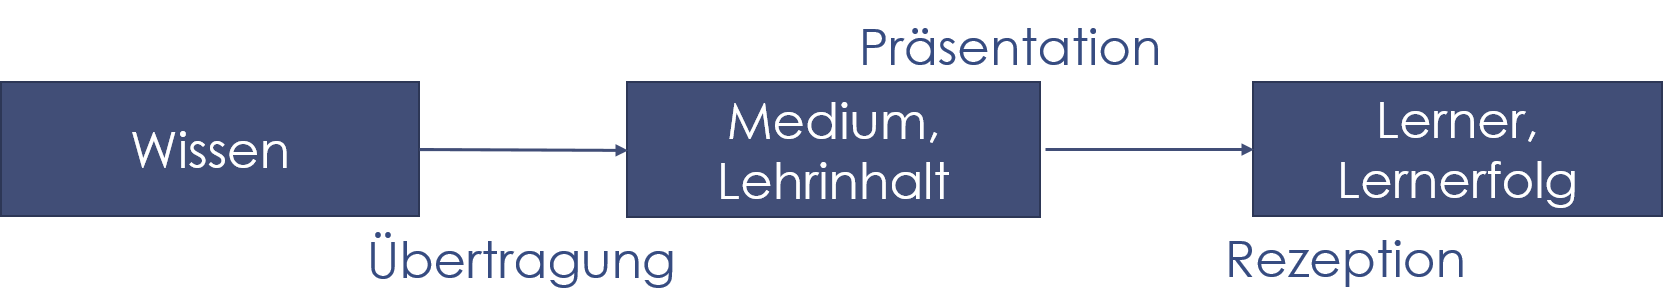
\includegraphics[width=0.7\textwidth]{Abbildungen/Kopiermodell.PNG}
	\caption{Medien als Übermittler von Lehrinhalten. \cite[S. 146]{Kerres.2001}}
	\label{fig:Kerres2001_Kopiermodell}
\end{figure}
Gemäß dem Kopiermodell (siehe Graphik \ref{fig:Kerres2001_Kopiermodell})wird das zu erlernende "Wissen von Sachexpert/innen auf ein Medium übertragen werden und von da aus dem Lernenden präsentiert" \cite[S. 146]{Kerres.2001}. Dies führt zu der Annahme, dass das Medium und nicht der Lehrende präsentiert. Außerdem impliziert es die Gleichheit von Lehr- und Wissensinhalten. %Wird das aus dem Lernende .... auf ein Mediuam übertragen werden --> Klingt seltsam

Der Name 'Kopiermodell' resultiert daraus, dass nach diesem didaktischen Modell, Lernen nur das Kopieren von Wissen in das Gedächtnis darstellt und eine derartige 1:1 Kopie möglich und sinnvoll ist. \cite[S. 145 f.]{Kerres.2001}

\subsection{Lernen durch Anregung}
\label{sub:LernenDurchAnregung}
\begin{figure}[h]
	\centering
	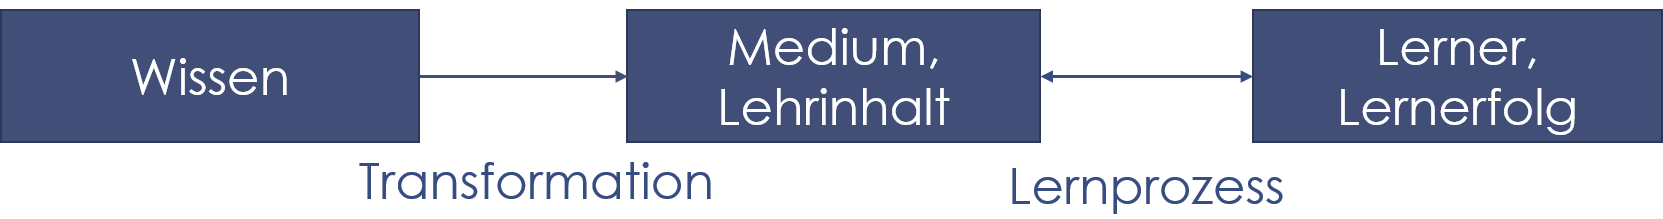
\includegraphics[width=0.7\textwidth]{Abbildungen/Anregungsmodell.PNG}
	\caption{Medien als Angebot zur Anregung von Lernprozessen. \cite[S. 147]{Kerres.2001}}
	\label{fig:Kerres2001_LernenDurchAnregung}
\end{figure}
Das Kopiermodell gilt aufgrund neuer Erkenntnisse über die menschliche Art zu Lernen und Informationen aufzunehmen als veraltet.
In dem nun beschriebenen alternativen Modell sollen die Lernmedien vielmehr das aktive Lernen anregen, als nur die Lerninhalte wiederzugeben. 
Dazu wird das zu vermittelnde Wissen eben in diese anregende Form transformiert. (siehe Graphik \ref{fig:Kerres2001_LernenDurchAnregung}) Diese Form soll neben der einfachen Aufnahme des Wissens auch zur Interaktion mit Mitlernenden und zur eigenen Aktion aufrufen. Beides führt zu einer intensiveren Auseinandersetzung mit dem Lernstoff. \cite[S. 147 f.]{Kerres.2001}